\documentclass[lettersize,journal]{IEEEtran}
\usepackage{amsmath,amsfonts}
\usepackage{algorithmic}
\usepackage{array}
\usepackage[caption=false,font=normalsize,labelfont=sf,textfont=sf]{subfig}
\usepackage{textcomp}
\usepackage{stfloats}
\usepackage{longtable}
\usepackage{url}
\usepackage{verbatim}
\usepackage{graphicx}
\hyphenation{op-tical net-works semi-conduc-tor IEEE-Xplore}
\def\BibTeX{{\rm B\kern-.05em{\sc i\kern-.025em b}\kern-.08em
    T\kern-.1667em\lower.7ex\hbox{E}\kern-.125emX}}
\usepackage{balance}
\begin{document}
\title{A Broadband Power Amplifier for 3GHz to 6GHz
Range in 130nm CMOS Technology}
\author{Uroš Minoski, 2023/30133}

\maketitle

\begin{abstract}
This paper presents the design and analysis of a broadband power amplifier operating in the frequency range from 3 GHz to 6 GHz using 130nm CMOS technology. The amplifier is coupled with a bandpass filter, employing Chebyshev and Bode-Fano design methodologies. The impact of transistor oxide thickness on amplifier performance is investigated, and simulations are carried out to optimize the design for maximum power output and linearity. The proposed amplifier demonstrates promising results, making it suitable for various wireless communication applications.
\end{abstract}

\begin{IEEEkeywords}
Broadband, power amplifier, bandpass filter, Chebyshev, Bode-Fano, CMOS technology.
\end{IEEEkeywords}

\section{Introduction}
The demand for broadband wireless communication systems has fueled the need for high-performance power amplifiers operating in a wide frequency range. In this context, the design of a broadband power amplifier becomes crucial for achieving efficient and reliable communication. This paper focuses on the development of a broadband power amplifier targeting the frequency band from 3 GHz to 6 GHz.


The design of the proposed amplifier involves the integration of a bandpass filter to mitigate unwanted harmonics and improve overall linearity. Two different filter designs, based on Chebyshev and Bode-Fano methodologies, are analyzed to compare their impact on amplifier performance. Additionally, the influence of transistor oxide thickness on the amplifier's characteristics is investigated.

The remainder of this paper is organized as follows: Section II presents the design of the matching network, including the use of Chebyshev and Bode-Fano filters. Section III discusses the design of the broadband power amplifier, considering the impact of transistor oxide thickness and provides simulation results and analysis, and Section IV concludes the paper with insights into potential future work.


\section{The Design of Matching Network}

Bode and Fano discovered that regardless of the matching
conditions used, the matching network and RC load system
must satisfy the inequality
%
\begin{equation}
	\label{eq:bode-fano}
	\int_0^{+\infty} \ln \left( \frac{1}{|\Gamma|} \right) d w \leq \frac{\pi}{R C},
\end{equation}
%
where $\Gamma$ is the reflection coefficient, and RC depends on
technology. Equation (\ref{eq:bode-fano}) shows that an increase in bandwidth
leads to an increase in the maximum reflection coefficient in
the bandpass.

The Chebyshev filter provides the most efficient system in
terms of Equation \ref{eq:bode-fano}. Therefore, Chebyshev filter design will
be used in the design of matching networks.

Two matching networks are analyzed, as shown in Fig. \ref{fig:prototype}.
The first network has Chebyshev Type I filter characteristics
and is driven by a generator with finite internal impedance.
The second network is designed using the Fano method and is
driven by a current generator with infinite internal impedance.

\subsection{Prototype Chebyshev Filter}

The Chebyshev attenuation function $A(w) = |H(w)|^{-2}$ is given by
%
\begin{equation}
	\label{eq:cheb_funct}
	A(w) = 1 + \epsilon^2 T_n^2(w),
\end{equation}
%
where
%
\begin{equation}
	T_n(w) = 
     \begin{cases}
        \cosh \left( n \, \cosh^{-1} w \right) & |w| \geq 1, \\
        \cos \left( n \, \cos^{-1} w \right) & |w| < 1,
     \end{cases}
\end{equation}
%
and $n$ is the order of filter.

If we define the ripple coefficient $\gamma$ as
%
\begin{equation}
	\label{eq:gamma_def}
	\gamma = \sinh \left( \frac{1}{n} \sinh^{-1} \epsilon^{-1} \right),
\end{equation}
%
filter elements $g_i$, for $r = 1, 2, ..., n - 1$, can be expressed as 
%
\begin{subequations} \label{eq:gi_all}
    \begin{align}
       g_r g_{r + 1} &= \frac{4 \sin \frac{(2 r + 1) \pi}{2n} \sin \frac{(2e - 1) \pi}{2n}}{\gamma^2 + \sin^2 \frac{r \pi}{n}} \label{eq:gi_grgr+1} \\
        g_n &= \frac{2 \sin \frac{\pi}{2n}}{\gamma} \label{eq:gi_gn} 
    \end{align}
\end{subequations}


By substituting $n = 3$ into equations (\ref{eq:gi_grgr+1}) and (\ref{eq:gi_gn}) we get
%
\begin{subequations} \label{eq:gi_all_val}
	\begin{align}
		g_1 &= \frac{1}{\gamma} \label{eq:g1_val} \\
		g_2 &= \frac{\gamma}{\gamma^2 + \frac{3}{4}} \label{eq:g2_val} \\
		g_3 &= \frac{1}{\gamma} \label{eq:g3_val} 
	\end{align}
\end{subequations}

Since the minimum and maximum attenuations in the passband are $A_{min} = 0$ and $A_{max} = 1 + \epsilon^2$, ripple in passband is equal to
%
\begin{equation}
	\label{eq:cheb_ripple}
	\delta = 10 \log_{10} \left( 1 + \epsilon^2 \right),
\end{equation}
%
where $\epsilon$ can be expressed by finding the inverse function of (\ref{eq:gamma_def}) as 
%
\begin{equation}
	\label{eq:epsilon}
	\epsilon = \sinh^{-1} \left( n \sinh^{-1} \gamma \right).
\end{equation}


For a fixed $\gamma = 1$ and $n = 3$, ripple in the passband is $\delta = 0.0877 \, \text{dB}$.

\begin{figure}[!t]
\centering
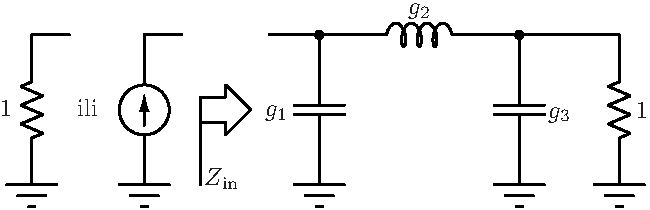
\includegraphics[width=3.4in]{./fig/prototype.pdf}
\caption{Prototype matching networks. One is driven by a generator with finite,
and the other with infinite internal impedance.}
\label{fig:prototype}
\end{figure}

\subsection{Prototype Fano Matching Network}

In the case of the Fano design method of a network driven by a generator with an infinite internal impedance, equations
(\ref{eq:gi_grgr+1}) and (\ref{eq:gi_gn}) become
%
\begin{subequations} \label{eq:gi_all_fano}
    \begin{align}
       g_r g_{r + 1} &= \frac{4 \sin \frac{(2 r + 1) \pi}{2n} \sin \frac{(2e - 1) \pi}{2n}}{2x^2(1 - \cos\frac{r\pi}{n}) + \sin^2\frac{r\pi}{n}} \label{eq:gi_grgr+1_fano} \\
        g_n &= \frac{\sin \frac{\pi}{2n}}{x}, \label{eq:gi_gn_fano} 
    \end{align}
\end{subequations}
%
for $r = 1, 2, ..., n - 1$. By substituting $n = 3$ into equations (\ref{eq:gi_grgr+1_fano}) and (\ref{eq:gi_gn_fano}) we get
%
\begin{subequations} \label{eq:gi_all_val_fano}
	\begin{align}
		g_1 &= \frac{12 x^2 + 3}{8x^2 + 6x} \label{eq:g1_val_fano} \\
		g_2 &= \frac{16x}{3 \cdot (4x^2 + 1)} \label{eq:g2_val_fano} \\
		g_3 &= \frac{1}{2x} \label{eq:g3_val} 
	\end{align}
\end{subequations}

Ripple in the passband can be found to be 
%
\begin{equation}
	\label{eq:ripple_fano}
	\delta = 10 \log_{10} \left( \coth^2 \left( n \sinh^{-1} x \right) \right).
\end{equation}

For a fixed $x = 1$ and $n = 3$, ripple in the passband is $\delta = 0.877 \, \text{dB}$.

\begin{figure}[!t]
\centering
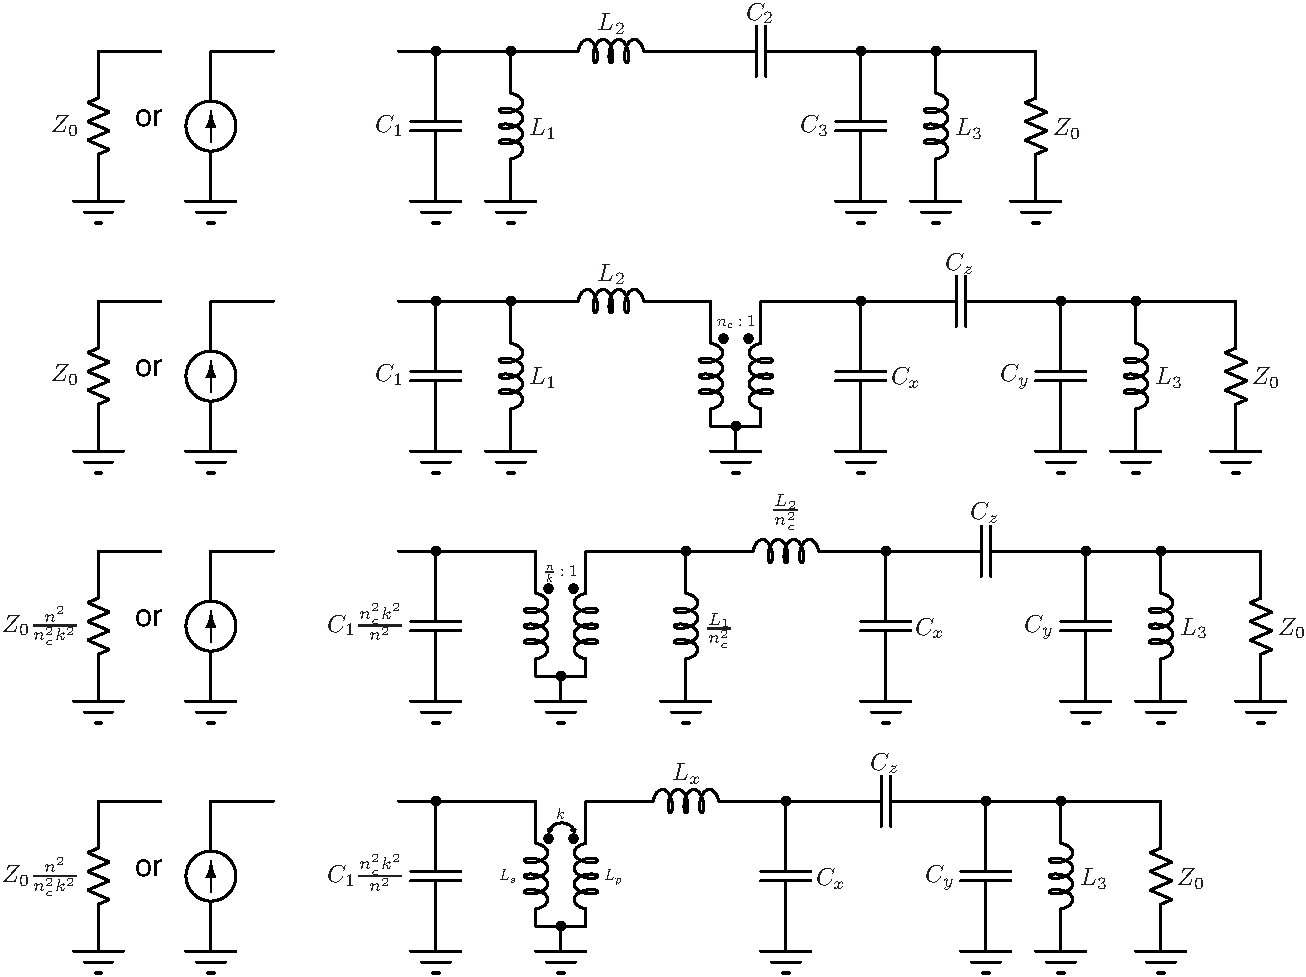
\includegraphics[width=3.4in]{./fig/denormalized_filter.pdf}
\caption{a) Denormalized bandpass filter. b) Norton transformation of capacitors
C2 and C3 . c) Moving an ideal transformer in front of inductor L1 . d)
Changing an ideal with a real transformer.}
\label{fig:denormalized_filter}
\end{figure}

\subsection{Denormalized Filter}

In order to get a bandpass filter out of the prototype, which is a lowpass filter normalized to $Z_0 = 1$ and cutoff frequency $w_0 = 1 \, \text{rad}$, we need to introduce a substitution
%
\begin{equation}
	\label{eq:subt}
	s \to \frac{s^2 + w_0^2}{s \Delta w_0},
\end{equation}
%
where $w_0$ is the central frequency, and $\Delta$ is the relative bandwidth.

The substitution (\ref{eq:subt}) suggests that capacitors and inductors from Fig. \ref{fig:prototype} transform into parallel and series oscillators, respectively, as shown in Fig. \ref{fig:denormalized_filter}.a.

Now we need to denormalize for input/output impedance $Z_0$. This is done by multiplying all impedances by $Z_0$ , which
means multiplying inductances by $Z_0$ and capacitances by $\frac{1}{Z_0}$.

Values of capacitors and inductors are
%
\begin{subequations} \label{eq:denom_all}
	\begin{align}
		C_1 &= \frac{g_1}{\Delta w_0 Z_0}, & L_1 &= \frac{\Delta Z_0}{w_0 g_1} \label{eq:denom_1} \\
		C_2 &= \frac{\Delta}{g_2 w_0 Z_0}, & L_2 &= \frac{g_2 Z_0}{w_0 \Delta} \label{eq:denom_2} \\
		C_3 &= \frac{g_3}{\Delta w_0 Z_0}, & L_2 &= \frac{\Delta Z_0}{w_0 g_3} \label{eq:denom_3}
	\end{align}
\end{subequations}

In order to scale input impedance by a factor of $n_c^{-1}$ we do Norton transformation under capacitors $C_2$ and $C_3$ , as shown in Fig. \ref{fig:denormalized_filter}.a. Transformation leads to Fig. \ref{fig:denormalized_filter}.b, where transformed capacitances are
%
\begin{subequations} \label{eq:norton_all}
	\begin{align}
		C_x &= n_c (n_c - 1) C_2 \label{eq:norton_x} \\
		C_y &= (1 - n_c) C_2 + C_3 \label{eq:norton_y} \\
		C_z &= n_c C_2 \label{eq:norton_z}
	\end{align}
\end{subequations}
%
For the transformation to be valid, or equivalently, for circuits from Fig. \ref{fig:denormalized_filter}.a and \ref{fig:denormalized_filter}.b to be considered equivalent, the following condition must hold true
%
\begin{equation}
	\label{eq:norton_cond}
	n_c \leq 1 + \frac{C_3}{C_2}.
\end{equation}

Next step is removal of ideal transformator towards the input. By doing that impidances and inductancces must be corrected by a factor of $n_c^{-2}$ and capacitances by $n_c^2$, as showrn in Fig. \ref{fig:denormalized_filter}.c.

Having a transformator is a requierment. To achive this, another ideal transformator is placed between first capacitor and first inductor, Fig. \ref{fig:denormalized_filter}.c. By doing so, impedances to the left of an ideal transforamtor must be corrected by factor of $n_c^2$.

The mathematical model of a real transformer comprises an ideal transformer, leakage and magnetic inductances. It is evident that $\frac{L_1}{n_c^2}$ and $\frac{L_2}{n_c^2}$ conform to this structure. Consequently, we obtain a real transformer, Fig. \ref{fig:denormalized_filter}.d, with
%
\begin{subequations} \label{eq:trans_all}
	\begin{align}
		L_p &= \frac{L_1}{k^2 n_c^2} \label{eq:trans_p} \\
		L_s &= L_p n^2 \label{eq:trans_s} \\
	    L_x &= \frac{k^2(L_1 + L_2) - L_1}{k^2 n_c^2} \label{eq:trans_x}
	\end{align}
\end{subequations}
%
where $L_p$ is inductance at primar, $L_s$ at secundar and $L_x$ is leakage inductance.

If we substitute equations (\ref{eq:denom_all}) into (\ref{eq:norton_all}) and (\ref{eq:trans_all}) we will get the complit set of equations for elements of a filter from Fig. \ref{fig:denormalized_filter}.d
%
\begin{subequations} \label{eq:all}
	\begin{align}
		Z_in &= \frac{Z_0 n^2}{k^2 n_c^2}, \label{eq:zin} \\
		C_1 &= \frac{g_1 k^2 n_c^2}{Z_0 \Delta w_0 n^2}, \label{eq:c1} \\
	    L_p &= \frac{Z_0 \Delta}{w_0 g_1 k^2 n_c^2}, \label{eq:lp} \\
	    L_s &= \frac{Z_0 \Delta n^2}{w_0 g_1 k^2 n_c^2}, \label{eq:lp} \\
	    L_x &= \frac{Z_0(\Delta^2(k^2 - 1) + g_1g_2k^2)}{\Delta w_0 g_1k^2n_c^2}, \label{eq:lx} \\
	    C_x &= \frac{\Delta n_c (n_c - 1)}{Z_0 w_0 g_2}, \label{eq:cx} \\
	    C_y &= \frac{g_2 g_3 - \Delta^2 (n_c^2 - 1)}{Z_0 \Delta w_0 g_2}, \label{eq:cy} \\
	    C_z &= \frac{\Delta n_c}{Z_0 w_0 g_2}, \label{eq:cz} \\
	    L_3 &= \frac{Z_0 \Delta}{w_0 g_3}, \label{eq:l3} \\
	\end{align}
\end{subequations}
%
where
%
\begin{equation}
	\label{eq:all_n}
	n = \sqrt{\frac{L_s}{L_p}}.
\end{equation}

From (\ref{eq:all}e) it can be seen that there is a condition for $k$ that satisfy $L_x = 0$. That condition is
%
\begin{equation}
	\label{eq:lx_cond}
	k = \sqrt{\frac{\Delta^2}{\Delta^2 + g_1 g_2}}, \,\,\,\,\, L_x = 0
\end{equation}

If we enforce $\gamma \geq 1$ for a filter exhibiting Chebyshev characteristics and $x \geq 1$ for a filter with current drive, and
choose $\Delta = \frac{\sqrt{2}}{2}$ , the corresponding minimum values for $k$ are
determined as follows
%
\begin{equation}
	\label{eq:k_min}
	k_{min, \gamma} = k_{min, x} = 0.5517.
\end{equation}

\begin{figure}[!t]
\centering
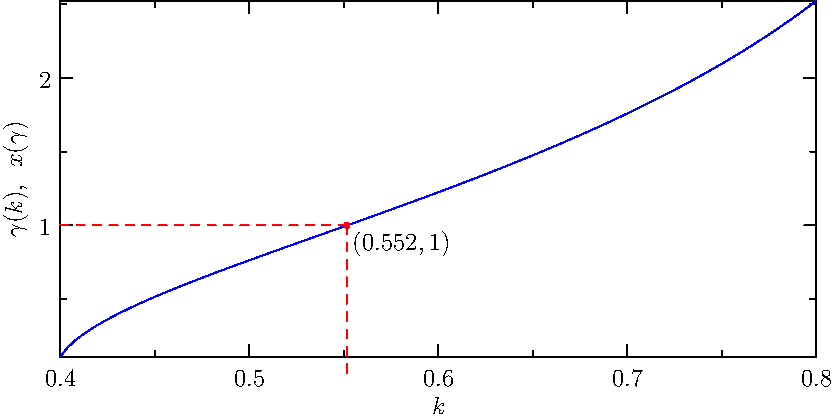
\includegraphics[width=3.4in]{./fig/gamma_function.pdf}
\caption{Functions $\gamma(k)$ and $x(k)$ for $\Delta = \frac{\sqrt{2}}{2}$.}
\label{fig:inverse_function_gamma}
\end{figure}

Inverse functions of (\ref{eq:lx_cond}) in termas of $\gamma$ and  $x$ when condition $L_x = 0$ is met are
%
\begin{equation}
	\label{eq:inverse_functions}
	\gamma(k, \Delta) = x(k, \Delta) = \frac{1}{2 \Delta} \sqrt{\frac{8 k^2 - 3  \Delta^2 (1 - k^2)}{1 - k^2}}.
\end{equation}
%
Fig. \ref{fig:inverse_function_gamma} shows $\gamma(k)$ and $x(k)$ for $\Delta = \frac{sqrt{2}}{2}$ . Minimum $k$ for which $\gamma$, or $x$ is greater then $0$, for same $\Delta$ is
%
\begin{equation}
	\label{eq:min_k}
	k_{min}|_{\gamma =0 , x = 0} = 0.3973.
\end{equation}

\section{The Design of Broadband Power Amplifier}

Power amplifier and bandpass filter are needed in order to to design a boradband power amplifier. Bandpass filters were designed in previous chapter. Their goal is to compensate parasitic capacitors of output stage of amplifier in frequency range of interest, in this case from $3 \, \text{GHz}$ to $6 \, \text{GHz}$.

In order to get maximum power amplification (for unit transistor amplifier) we have to match output impedance of $50 \, \Omega$ to optimal load impedance. We could also increase width of transistors to get higher power, but it has it's limits.

\begin{figure}[!t]
\centering
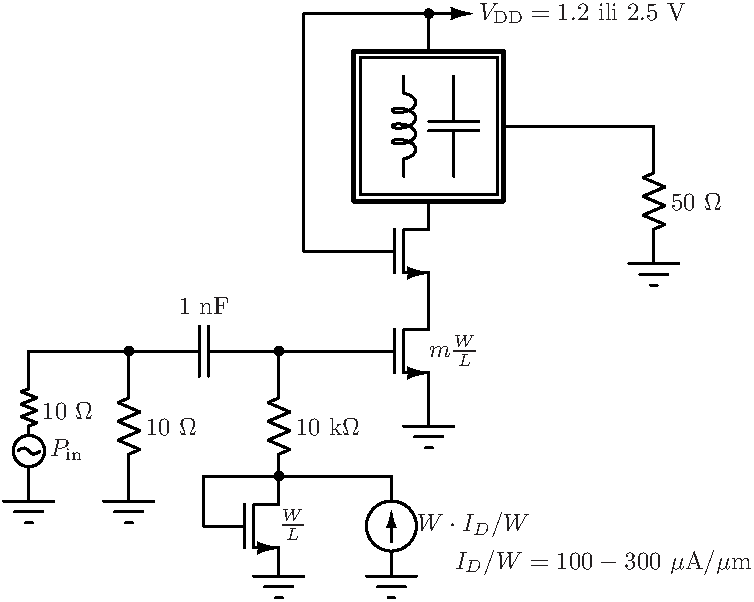
\includegraphics[width=3.4in]{./fig/blockpa.pdf}
\caption{Block diagram of power amplifier.}
\label{fig:blockPA}
\end{figure}

\subsection{Simulations and Results}
Simulations were conducted for two configurations of transistors in a cascode arrangement, Fig. \ref{fig:blockPA}. In the first configuration, both transistors have a similar oxide thickness, approximately $t_{ox} = 2.6 \, \text{nm}$. In this scenario, the width of the unit transistor is $20 \, \mu \text{m}$, and the current density is $192.23 \, \mu \text{A/} \mu \text{m}$. 

In the second configuration, the transistor at the output has a larger oxide thickness, approximately $t_{ox} = 7 \, \text{nm}$. In this case, the widths and current densities of the unit transistors are set to $20 \, \mu \text{m}$ and $252 \, \mu \text{A/} \mu \text{m}$ for $t_{ox} = 2.6 \, \text{nm}$, and $40 \, \mu \text{m}$ and $126 \, \mu \text{A/} \mu \text{m}$ for $t_{ox} = 7 \, \text{nm}$.

Simulations for finding parasitic capacitances at the output node, as well as for finding optimal capacitances are done with $20$ times the unit transistors. This implies that for the unit transistors, parasitic capacitances should be multiplied by $1/20$, optimal impedances and output power by $20$. 


\begin{figure}[!t]
\centering
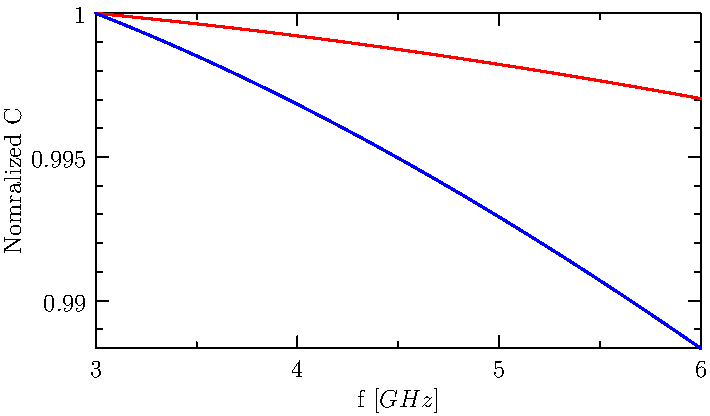
\includegraphics[width=3.4in]{./fig/Cd.pdf}
\caption{Relationship between output parasitic capacitance and frequency. The
red curve represents the scenario where both transistors possess a similar
oxide thickness, while the blue curve illustrates the case where the output
transistor has a larger oxide thickness. Simultaion is done for 20 times the
unit transistors.}
\label{fig:Cd}
\end{figure}

\begin{figure}[!t]
\centering
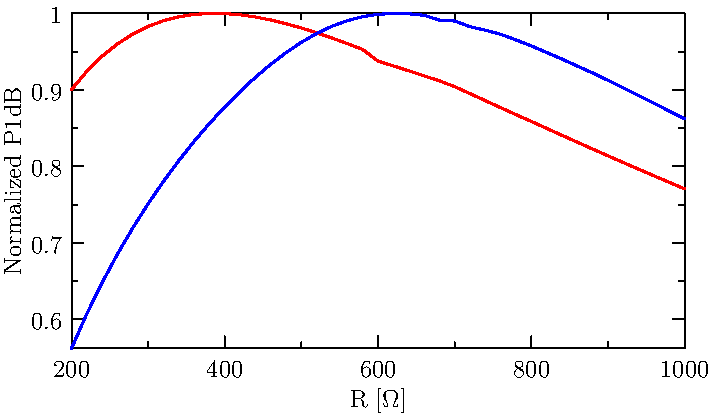
\includegraphics[width=3.4in]{./fig/Zopt.pdf}
\caption{Relationship between P1dB and load impedance. The red curve rep-
resents the scenario where both transistors possess a similar oxide thickness,
while the blue curve illustrates the case where the output transistor has a
larger oxide thickness. Simultaion is done for 20 times the unit transistors.}
\label{fig:Zopt}
\end{figure}

\begin{table}[b!]
\caption{Values of filter elements}

\footnotesize
  \begin{tabular}{ | l | c | c | c | c | c | c | r |}
    \hline
     & $Z_{in}$ [$\Omega$] & $C_1$ [pF] & $L_s$ [nF] & $L_p$ [nF] & $C_x$ [pF] & $C_z$ [pF] & $L_3$ [nF] \\ \hline
    Chebyshev & 15.21 & 3.49 & 0.403 & 0.403 & 3.49 & 1.52 & 1.33 \\ \hline
    Bode-Fano & 38.46 & 1.48 & 0.952 & 0.952 & 1.09 & 1.03 & 2.65 \\ \hline
  \end{tabular}
  \label{tab:all_elements}
\end{table}

Parasitic capacitance at the output of amplifier is found as
%
\begin{equation}
	\label{eq:cd}
	C_D = \frac{\Im \left\{ Y_{\text{out}} \right\}}{2 \pi f}, 
\end{equation}
%
where $Y_{out}$ is is admitance seen at the output of the amplifier. Fig. \ref{fig:Cd} shows normalized parasitic capacitance dpeandens on frequency, for both types of amplifier. We can see that the variation in parasitic capacitance remains quite minimal with respect to changes in frequency. Therefore, the selection of capacitance for the central frequency, $f = 3 \sqrt{2} \, \text{GHz}$, is deemed appropriate. Their values are
%
\begin{equation}
	\label{eq:cd_1}
	C_D = 17.97 \, \text{fF}
\end{equation}
%
for the first type of amplifier, featuring transistors with similar
oxide thicknesses, and
%
\begin{equation}
	\label{eq:cd_2}
	C_D = 23.13 \, \text{fF}
\end{equation}
%
for the second type of amplifier, characterized by transistors with different oxide thicknesses.


Optimal load impedences for which power gain is maximum can be found by simulating P1dB commpenstaion point for different valuse of resistors. Fig. \ref{fig:Zopt} shows P1dB dpeandens on load impedance for both types of amplifiers. The values of optimal impedances (for unit transistors) are
%
\begin{equation}
	\label{eq:Ropt_1}
	R_{opt} = 380 \, \Omega
\end{equation}
%
for the first type of amplifier, with transistors of similar oxide thicknesses, and
%
\begin{equation}
	\label{eq:Ropt_1}
	R_{opt} = 620 \, \Omega
\end{equation}
%
for the second type of amplifier, featuring transistors with different oxide thicknesses.



To maximize the output power, it is essential to utilize a transistor width multiplication factor that results in the minimum optimal impedance. This is because, in such a scenario, the multiplication factor attains its maximum value, and the output power is directly proportional to this factor. As depicted in Figure~\ref{fig:inverse_function_gamma}, the ripple is inversely proportional to $k$. Equation~(\ref{eq:zin}) further illustrates that $Z_{\text{in}}$ is inversely proportional to $k$. Consequently, for the minimum optimal impedance, the ripple reaches its maximum. Therefore, to achieve higher power, it is necessary to deliberately increase the ripple.


For $n_c = n_{c, \text{max}}$ and $L_x = 0$ and $n = 1$ and $k = k_{\text{min}} = 0.5512$, we obtain $Z_{\text{in, min}} = 15.21 \, \Omega$ with a multiplication factor $M = 25$ (for transistors with the same oxide thickness) and $M = 41$ (for transistors with different oxide thickness) for a filter with Chebyshev characteristics. Additionally, for Bode-Fano filter design, we have $Z_{\text{in, min}} = 38.46 \, \Omega$ and $M = 10$ (for transistors with the same oxide thickness) and $M = 16$ (for transistors with different oxide thickness).

Table~\ref{tab:all_elements} presents the values of all elements for filter with Chebyshev characteristics and filter designed with Bode-Fano method. 


\begin{table}[h!]
\caption{Values of capacitor $C_1$}
\footnotesize
\begin{center}
\begin{tabular}{ | c | c | c |}
    \hline
     & Same oxide thickness & Different oxide thickness \\ \hline
    Chebyshev & 3.04 pF & 2.54 pF \\ \hline
    Bode-Fano & 1.30 pF & 1.11 pF \\ \hline
  \end{tabular}
  \label{tab:c1}
\end{center}
\end{table}

\begin{table}[h!]
\caption{Maximum value of compression point}
\footnotesize
\begin{center}
\begin{tabular}{ | c | c | c |}
    \hline
     & Same oxide thickness & Different oxide thickness \\ \hline
    Chebyshev & 11.93 dBm & 21.19 dBm \\ \hline
    Bode-Fano &  7.26 dBm & 16.55 dBm \\ \hline
  \end{tabular}
  \label{tab:p1db}
\end{center}
\end{table}

\clearpage

The only distinguishing factor between amplifiers with transistors having the same and different oxide thickness is the value of the capacitor $C_1$. Due to the presence of parasitic capacitance at the output node, it is possible to integrate that capacitance into the capacitor $C_1$ of the filter. Table~\ref{tab:c1} presents the values of $C_1$ corresponding to each combination of filter and amplifier types.

Table~\ref{tab:p1db} displays the maximum P1dB values within the passband for each combination of filter and amplifier types. These values were measured for $k = k_{\text{min}} = 0.5512$.


Figures~\ref{fig:1v2_p1db_1} and \ref{fig:2v5_p1db_1} illustrate the P1dB values measured across the frequency range from 1 GHz to 10 GHz. It is evident that filters with Chebyshev characteristics (depicted by red lines) provide higher power in both cases. Furthermore, Figures~\ref{fig:1v2_p1db_2} and \ref{fig:2v5_p1db_2} showcase the ripple in the passband. It is clear that the filter designed using the Bode-Fano method (depicted by blue lines) exhibits a smoother response in the passband for both cases.

\begin{figure}[!t]
\centering
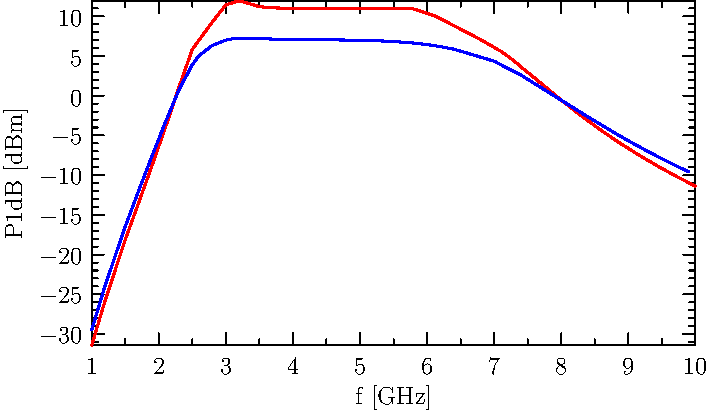
\includegraphics[width=3.4in]{./fig/1V2_P1dB_1.pdf}
\caption{The P1dB values are observed within the frequency range from 1 GHz to 10 GHz. The blue line corresponds to a filter designed using the Bode-Fano method, while the red line represents a filter exhibiting Chebyshev characteristics.}
\label{fig:1v2_p1db_1}
\end{figure}

\begin{figure}[!t]
\centering
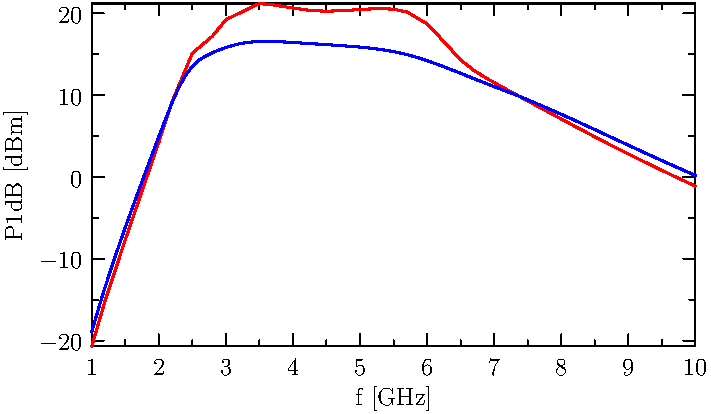
\includegraphics[width=3.4in]{./fig/2V5_P1dB_1.pdf}
\caption{P1dB values are measured across the frequency range of 1 GHz to 10 GHz for amplifiers with transistors having the different oxide thickness. The blue line represents a filter designed using the Bode-Fano method, while the red line corresponds to a filter exhibiting Chebyshev characteristics.}
\label{fig:2v5_p1db_1}
\end{figure}
 
\begin{figure}[!t]
\centering
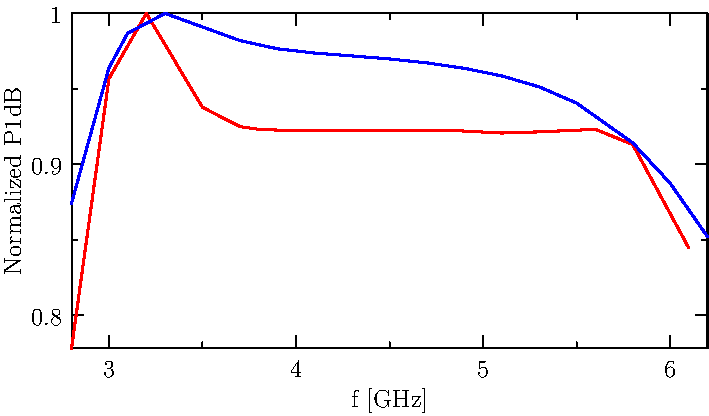
\includegraphics[width=3.4in]{./fig/1V2_P1dB_2.pdf}
\caption{The P1dB values are observed within the frequency range from 1 GHz to 10 GHz. The blue line corresponds to a filter designed using the Bode-Fano method, while the red line represents a filter exhibiting Chebyshev characteristics.}
\label{fig:1v2_p1db_2}
\end{figure}

\begin{figure}[!t]
\centering
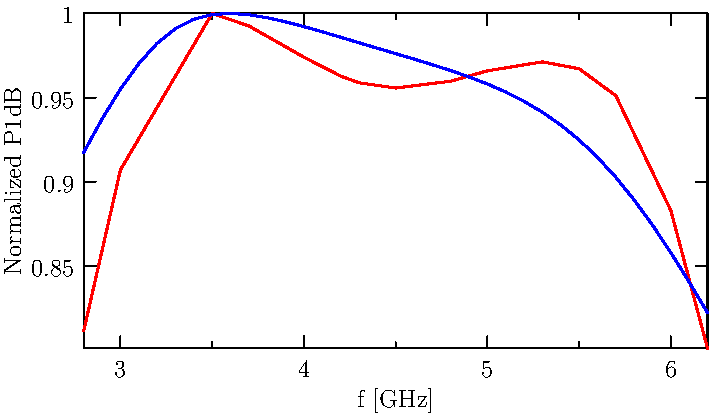
\includegraphics[width=3.4in]{./fig/2V5_P1dB_2.pdf}
\caption{P1dB values are measured across the frequency range of 1 GHz to 10 GHz for amplifiers with transistors having the different oxide thickness. The blue line represents a filter designed using the Bode-Fano method, while the red line corresponds to a filter exhibiting Chebyshev characteristics.}
\label{fig:2v5_p1db_2}
\end{figure}

\section{Conclusion}

This work presents a comprehensive study on the design of a broadband power amplifier in the 3GHz to 6GHz range, utilizing Chebyshev and Bode-Fano matching networks. Through analytical analysis and optimization, prototype filters were designed, considering ideal and real transformers for practical applications.

Simulations for various transistor configurations show competitive results in terms of P1dB compression point and power gain. The comparison between Chebyshev and Bode-Fano filters reveals the latter's advantages in passband ripple and frequency response smoothness.

In summary, this research contributes valuable insights into the design of broadband power amplifiers. The presented methodology provides a foundation for further exploration, aiding in the development of high-performance communication systems. Future work may involve additional optimizations and practical implementations to enhance applicability in specific scenarios.

 

\end{document}


